\pagestyle{fancy}
\fancyhf{}
\fancyhead[R]{Appendices}
\renewcommand{\headrulewidth}{0.4pt}

\section*{Appendix A: Database Schema}

Table~\ref{tab:schema_queries} through Table~\ref{tab:schema_aggregates} document the complete database schema used by the application.

\begin{table}[H]
\centering
\caption{queries table}
\label{tab:schema_queries}
\small
\begin{tabularx}{\textwidth}{ll>{\raggedright\arraybackslash}X}
\toprule
\textbf{Column} & \textbf{Type} & \textbf{Description} \\
\midrule
id & VARCHAR(36) PK & UUID primary key \\
raw\_term & VARCHAR(255) & Original search term as entered by user \\
normalized\_term & VARCHAR(255) UNIQUE & Lowercased, accent-stripped, whitespace-collapsed \\
created\_at & TIMESTAMP & Creation timestamp \\
\bottomrule
\end{tabularx}
\end{table}

\begin{table}[H]
\centering
\caption{query\_runs table}
\label{tab:schema_query_runs}
\small
\begin{tabularx}{\textwidth}{ll>{\raggedright\arraybackslash}X}
\toprule
\textbf{Column} & \textbf{Type} & \textbf{Description} \\
\midrule
id & VARCHAR(36) PK & UUID primary key \\
query\_id & VARCHAR(36) FK & Reference to queries table \\
status & ENUM & pending, running, completed, failed \\
started\_at & TIMESTAMP & When the run was created \\
finished\_at & TIMESTAMP & When the run completed or failed \\
scope\_config & JSON & Subreddit list and other scope parameters \\
match\_strategy & VARCHAR(100) & Matching strategy name \\
language\_filter & VARCHAR(50) & Target content language code \\
data\_fresh\_until & TIMESTAMP & Cache expiry timestamp \\
error\_message & TEXT & Error details if status is failed \\
\bottomrule
\end{tabularx}
\end{table}

\begin{table}[H]
\centering
\caption{documents table}
\label{tab:schema_documents}
\small
\begin{tabularx}{\textwidth}{ll>{\raggedright\arraybackslash}X}
\toprule
\textbf{Column} & \textbf{Type} & \textbf{Description} \\
\midrule
id & VARCHAR(36) PK & UUID primary key \\
source\_type & ENUM & post or comment \\
source\_id & VARCHAR(36) & ID of the source post or comment \\
subreddit\_id & VARCHAR(36) FK & Reference to subreddits table \\
full\_text & TEXT & Complete text content \\
detected\_language & VARCHAR(20) & ISO language code from langdetect \\
language\_confidence & FLOAT & Detection confidence (0--1) \\
created\_utc & TIMESTAMP & Original Reddit creation time \\
score & INTEGER & Reddit score (upvotes minus downvotes) \\
permalink & TEXT & URL to original Reddit content \\
\bottomrule
\end{tabularx}
\end{table}

\begin{table}[H]
\centering
\caption{sentiment\_results table}
\label{tab:schema_sentiment}
\small
\begin{tabularx}{\textwidth}{ll>{\raggedright\arraybackslash}X}
\toprule
\textbf{Column} & \textbf{Type} & \textbf{Description} \\
\midrule
id & VARCHAR(36) PK & UUID primary key \\
query\_run\_id & VARCHAR(36) FK & Reference to query\_runs table \\
document\_id & VARCHAR(36) FK & Reference to documents table \\
provider\_name & VARCHAR(100) & Provider identifier (openai, mock) \\
provider\_version & VARCHAR(100) & Provider version string \\
label & ENUM & very\_negative, negative, neutral, positive, very\_positive \\
score\_value & INTEGER & $-2$ to $+2$ mapping \\
confidence & FLOAT & Classification confidence (0--1) \\
rationale & TEXT & Explanation in source language \\
evidence\_phrases & JSON & Array of 1--3 exact quotes \\
created\_at & TIMESTAMP & Classification timestamp \\
\bottomrule
\end{tabularx}
\end{table}

\begin{table}[H]
\centering
\caption{aggregates table}
\label{tab:schema_aggregates}
\small
\begin{tabularx}{\textwidth}{ll>{\raggedright\arraybackslash}X}
\toprule
\textbf{Column} & \textbf{Type} & \textbf{Description} \\
\midrule
id & VARCHAR(36) PK & UUID primary key \\
query\_run\_id & VARCHAR(36) FK & Reference to query\_runs table \\
aggregate\_type & ENUM & overview, sentiment\_distribution, sentiment\_timeline, volume\_timeline, subreddit\_breakdown, sentiment\_heatmap, rolling\_sentiment\_timeline, phrase\_breakdown, spike\_events \\
payload & JSON & Precomputed chart data \\
created\_at & TIMESTAMP & Aggregation timestamp \\
\bottomrule
\end{tabularx}
\end{table}

\section*{Appendix B: API Endpoint Reference}

Table~\ref{tab:api_endpoints} lists the REST API endpoints exposed by the FastAPI backend.

\begin{table}[H]
\centering
\caption{API endpoint reference}
\label{tab:api_endpoints}
\small
\begin{tabularx}{\textwidth}{ll>{\raggedright\arraybackslash}X}
\toprule
\textbf{Method} & \textbf{Path} & \textbf{Description} \\
\midrule
POST & /queries & Create a new query and run (or return cached result) \\
GET & /query-runs/\{run\_id\} & Get status and metadata of a query run \\
GET & /query-runs/\{run\_id\}/charts & Get precomputed chart payloads \\
GET & /query-runs/\{run\_id\}/documents & Get matched documents with sentiment details \\
POST & /query-runs/\{run\_id\}/refresh & Force a fresh re-run \\
POST & /subreddits/validate & Validate subreddit names against Reddit \\
GET & /ready & Health check endpoint \\
\bottomrule
\end{tabularx}
\end{table}

\section*{Appendix C: Dashboard Screenshots}

\begin{figure}[H]
    \centering
    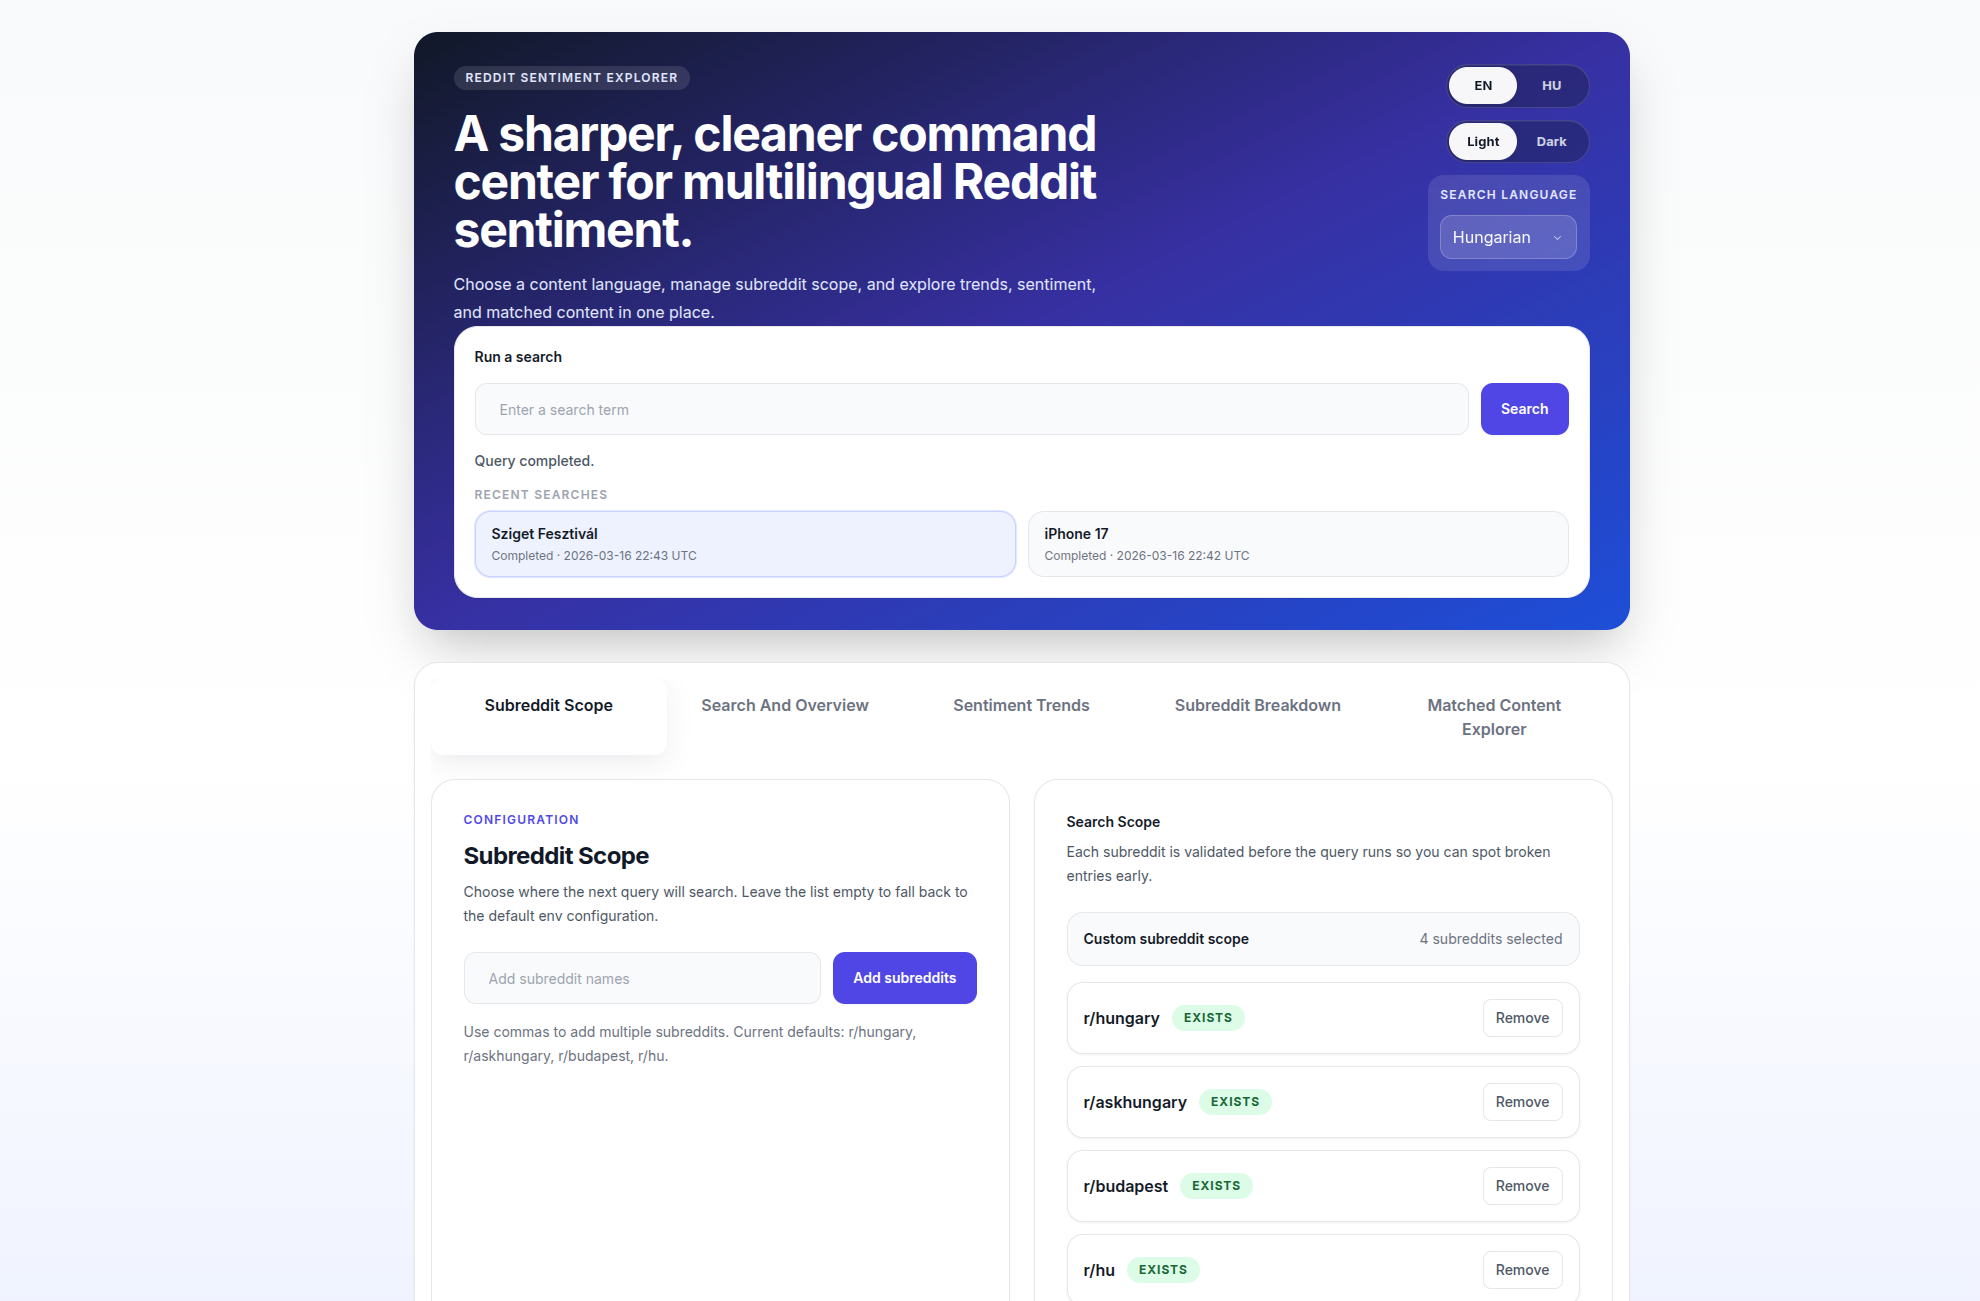
\includegraphics[width=\textwidth]{figures/dashboard-hero.png}
    \caption{Dashboard landing page with search interface and subreddit scope management.}
    \label{fig:appendix_dashboard}
\end{figure}

\begin{figure}[H]
    \centering
    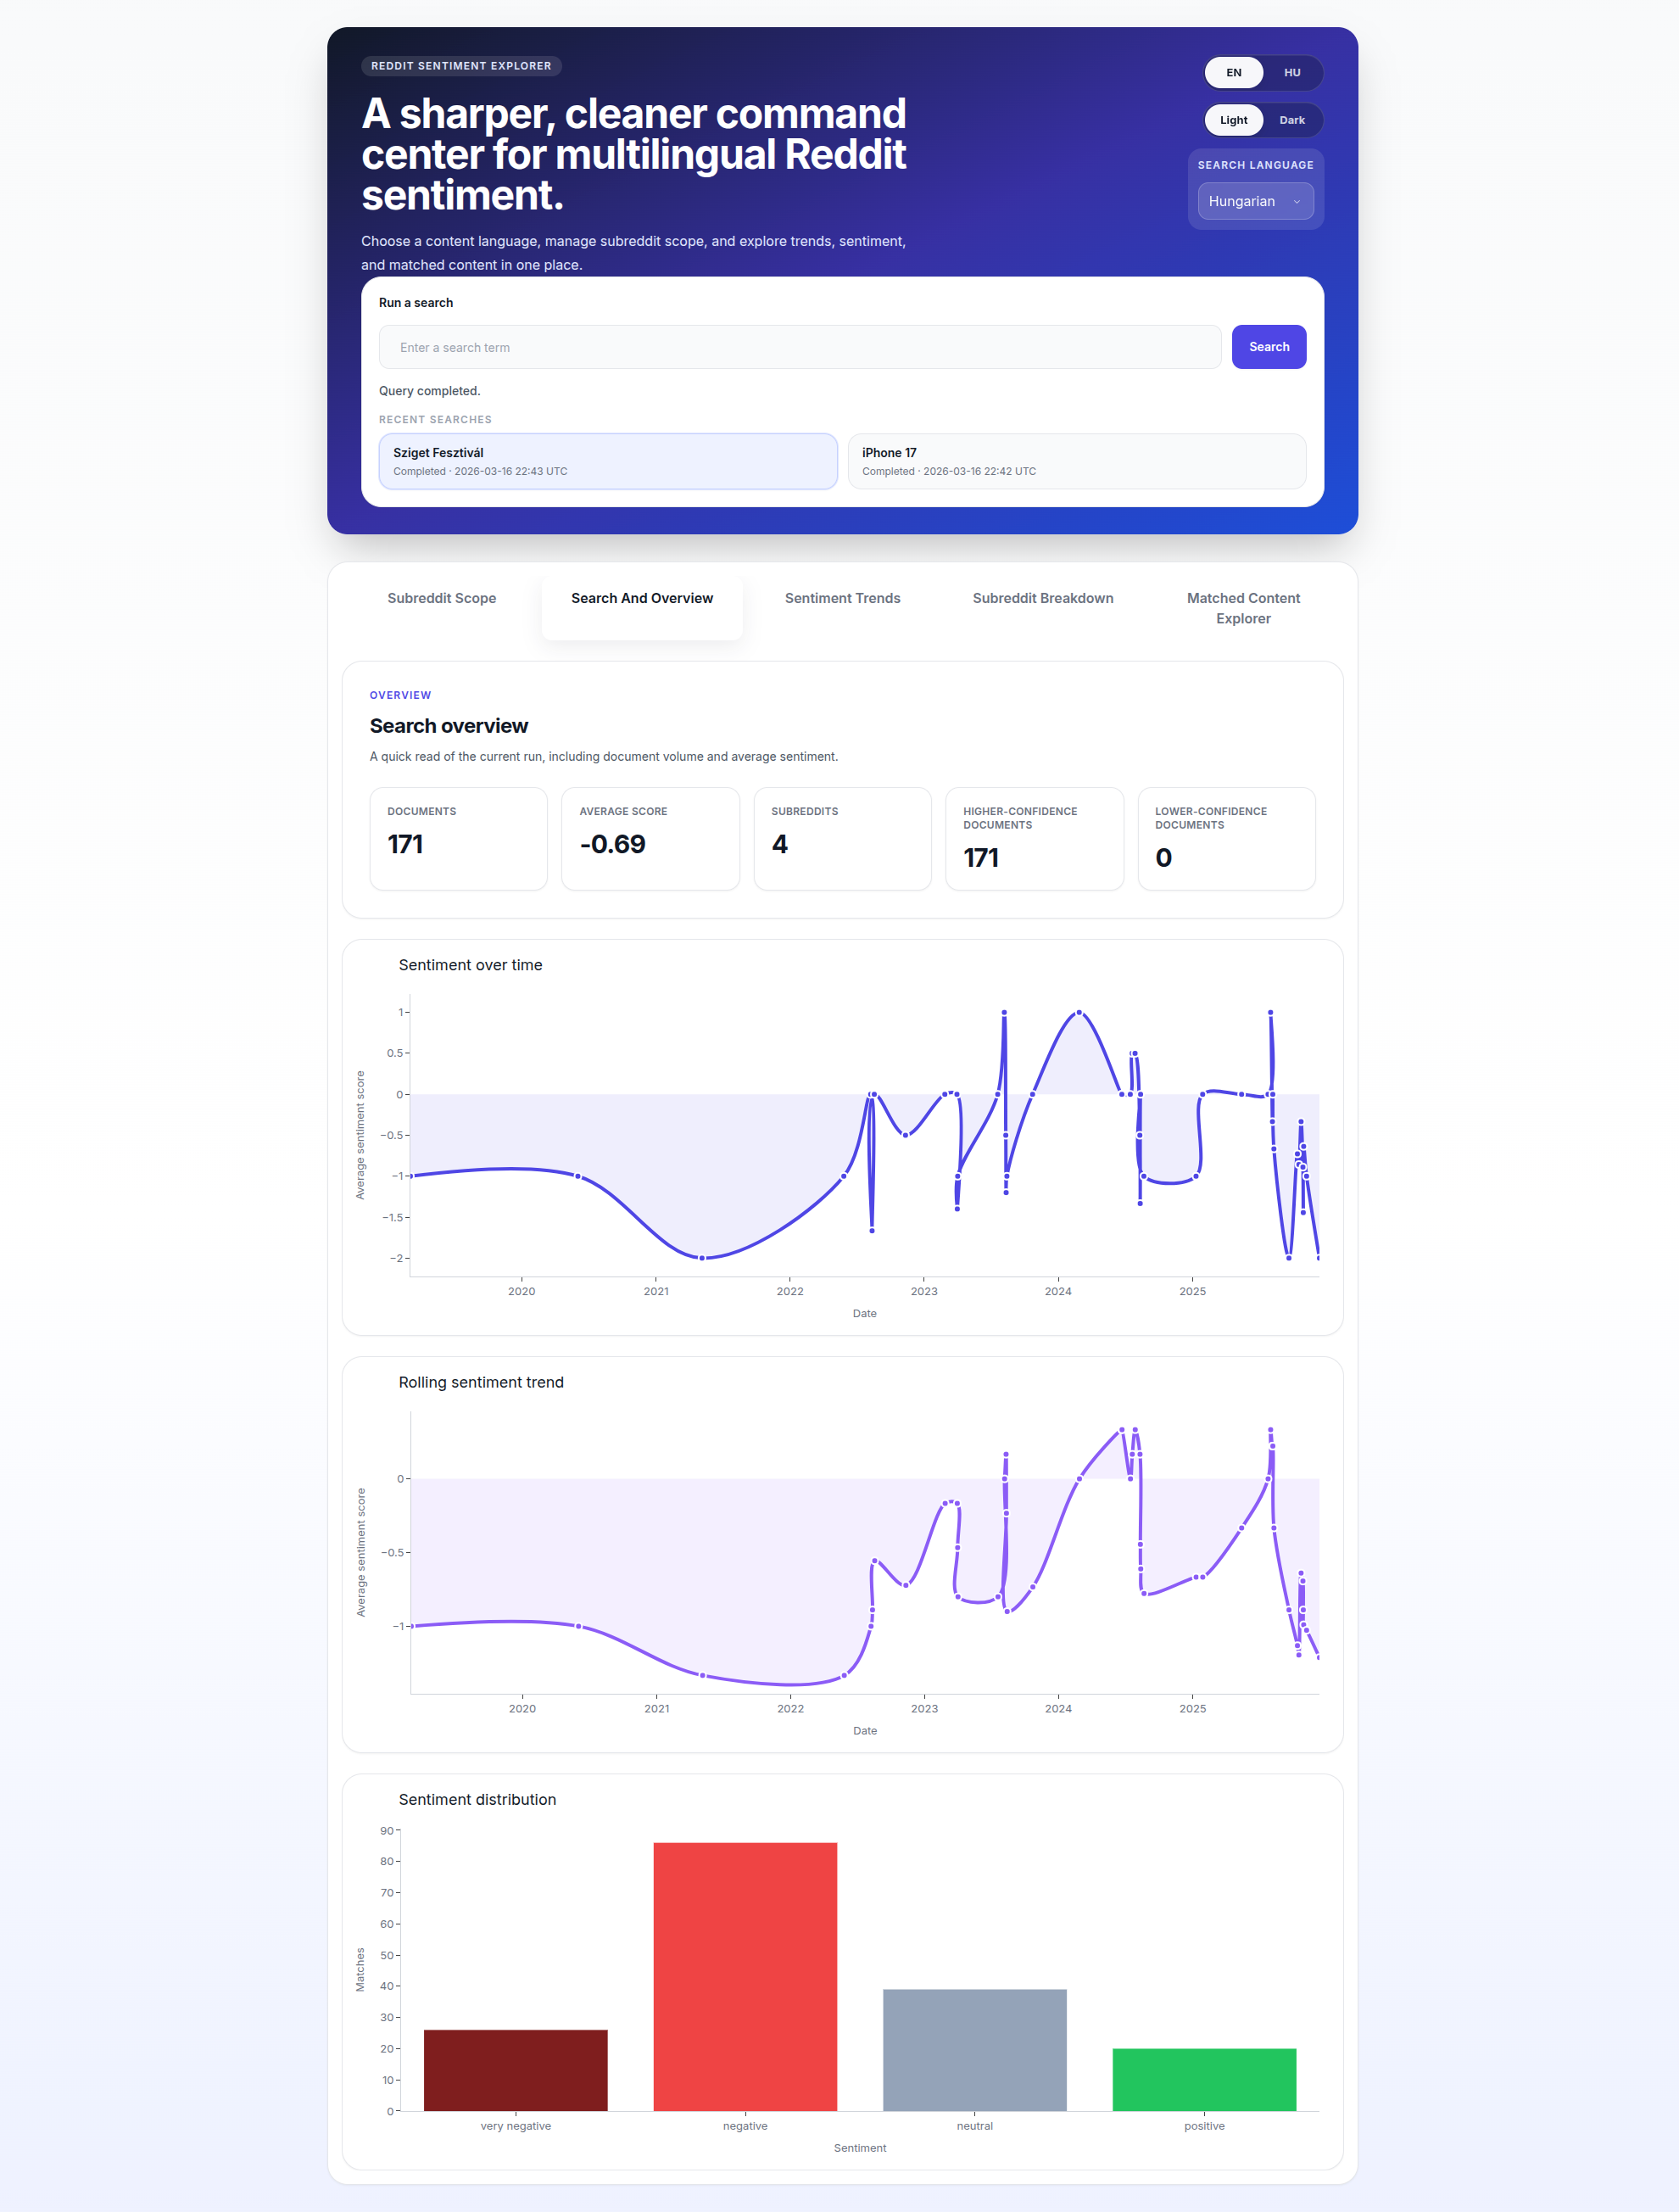
\includegraphics[width=\textwidth]{figures/search-overview.png}
    \caption{Search And Overview tab with overview metrics, sentiment timeline, rolling sentiment trend, and sentiment distribution charts.}
    \label{fig:appendix_overview}
\end{figure}

\begin{figure}[H]
    \centering
    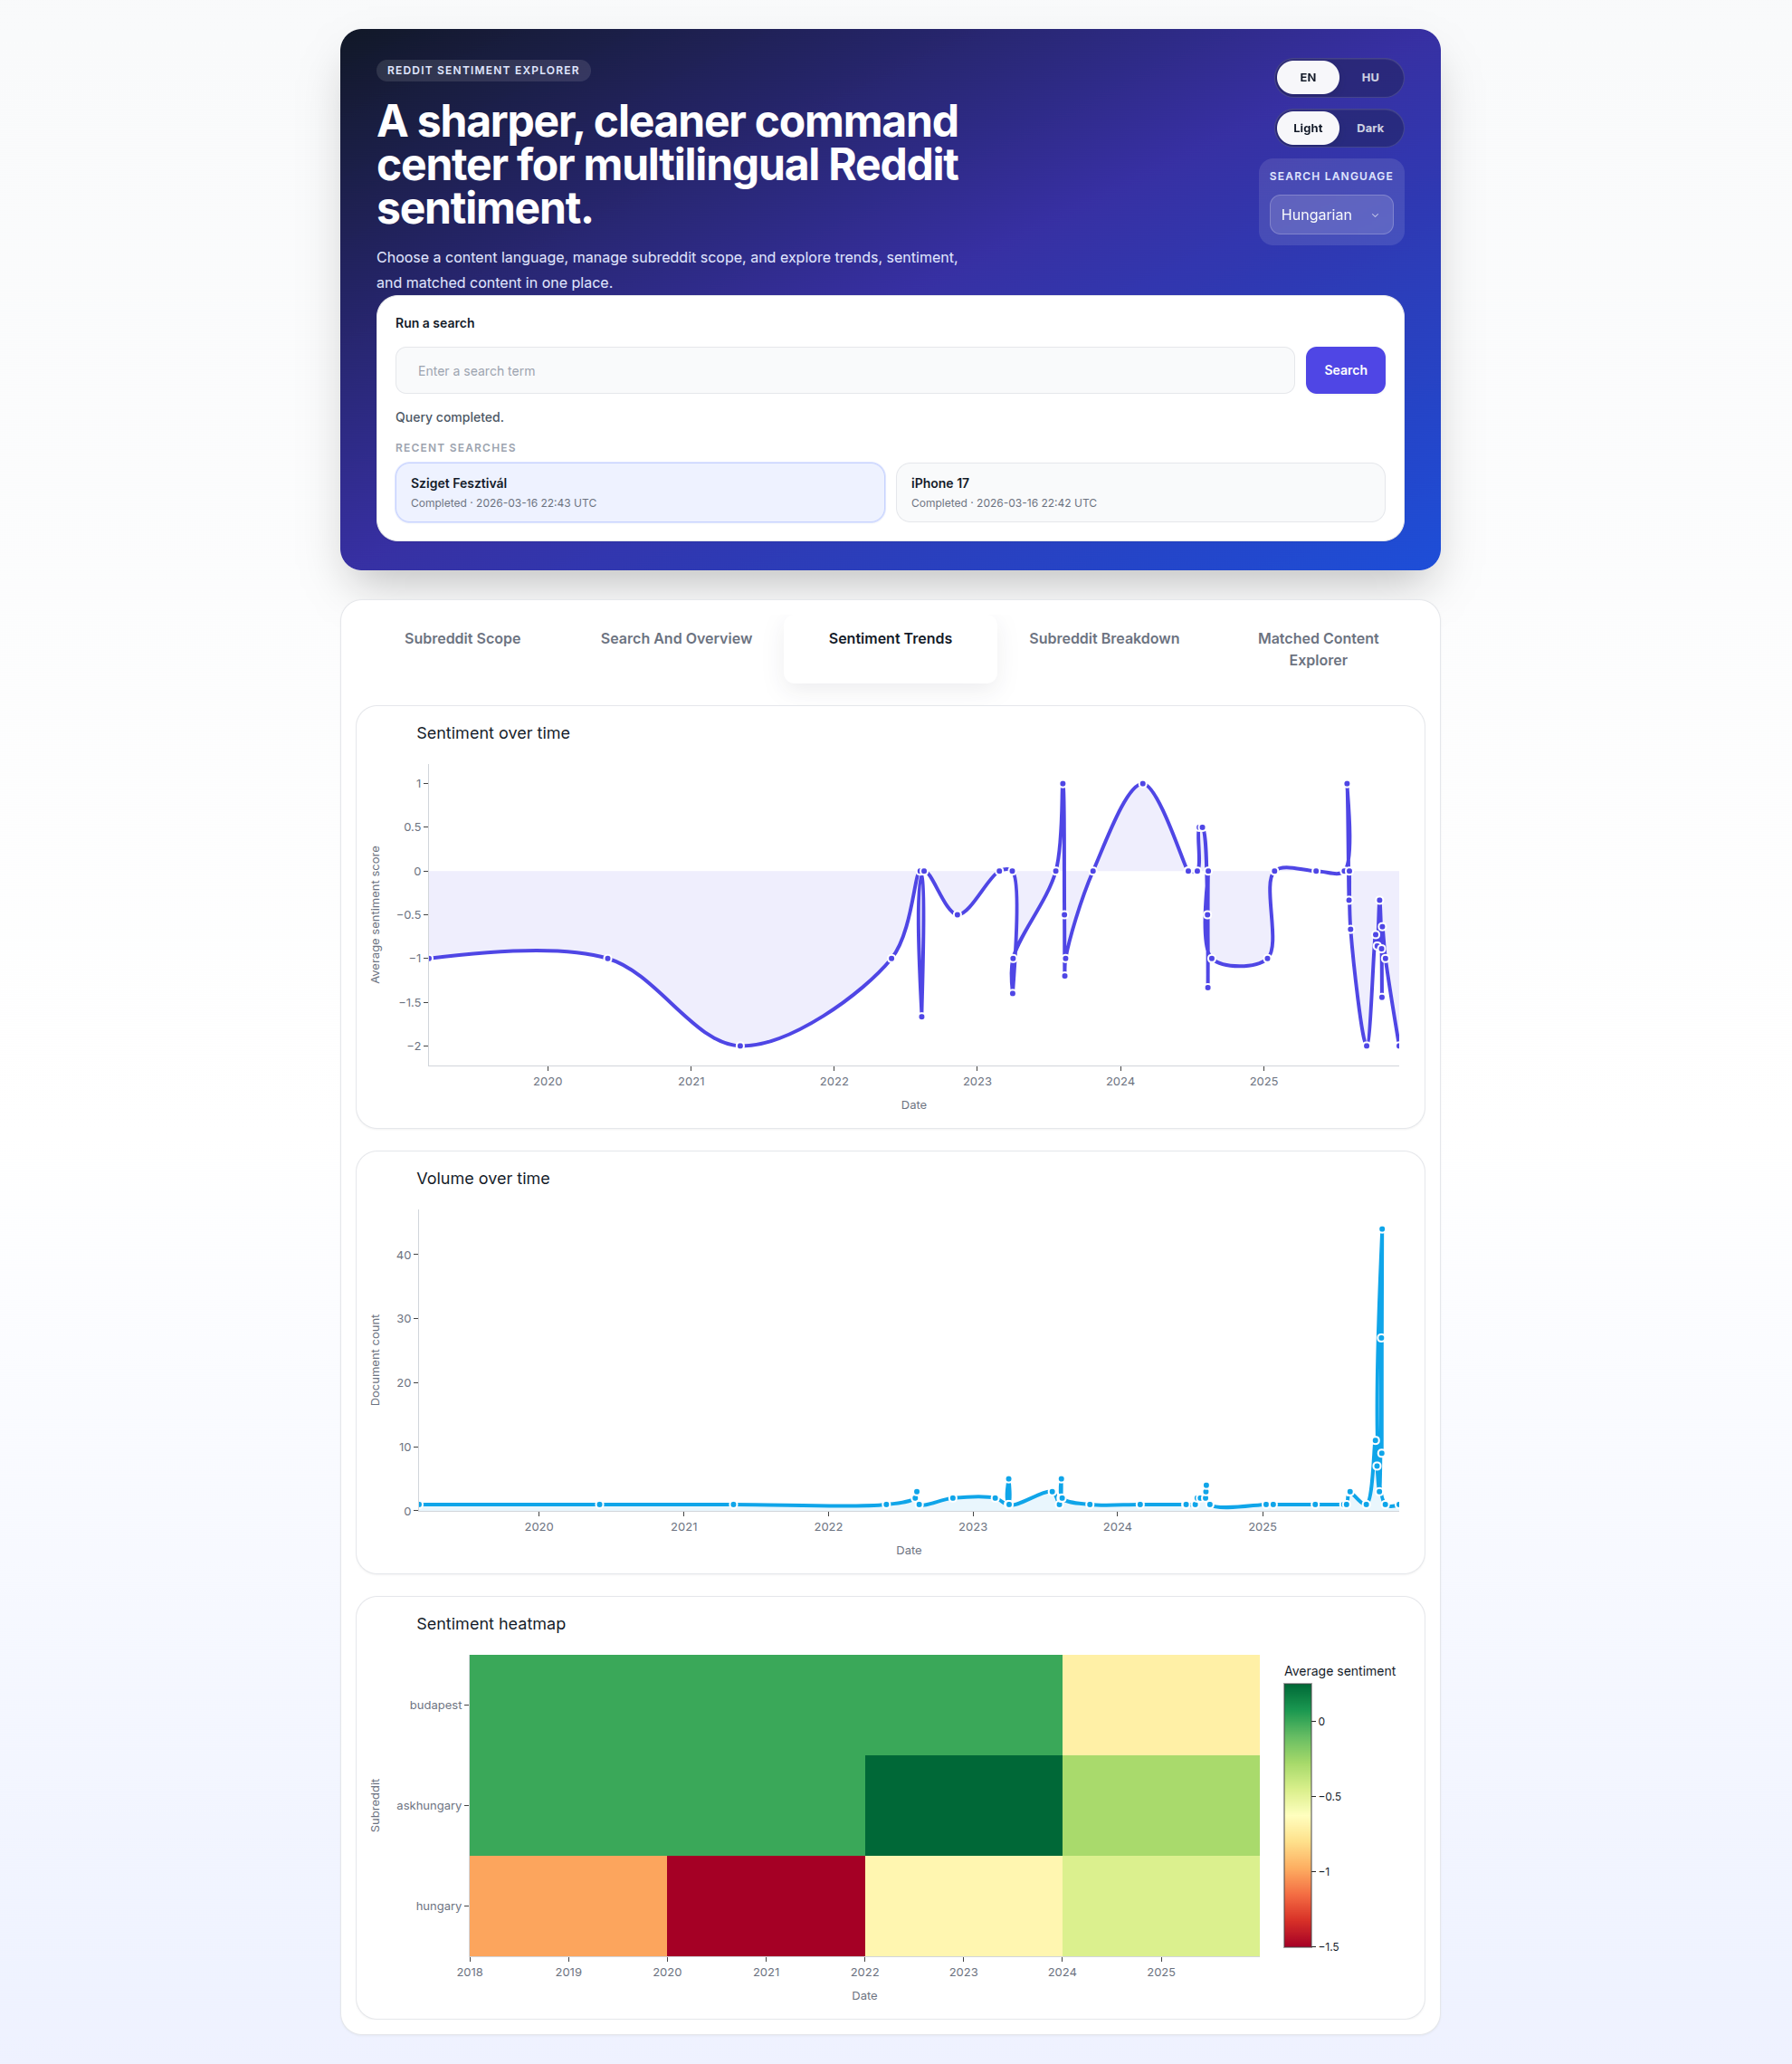
\includegraphics[width=\textwidth]{figures/sentiment-trends.png}
    \caption{Sentiment Trends tab with sentiment timeline, volume timeline, and sentiment heatmap.}
    \label{fig:appendix_trends}
\end{figure}

\begin{figure}[H]
    \centering
    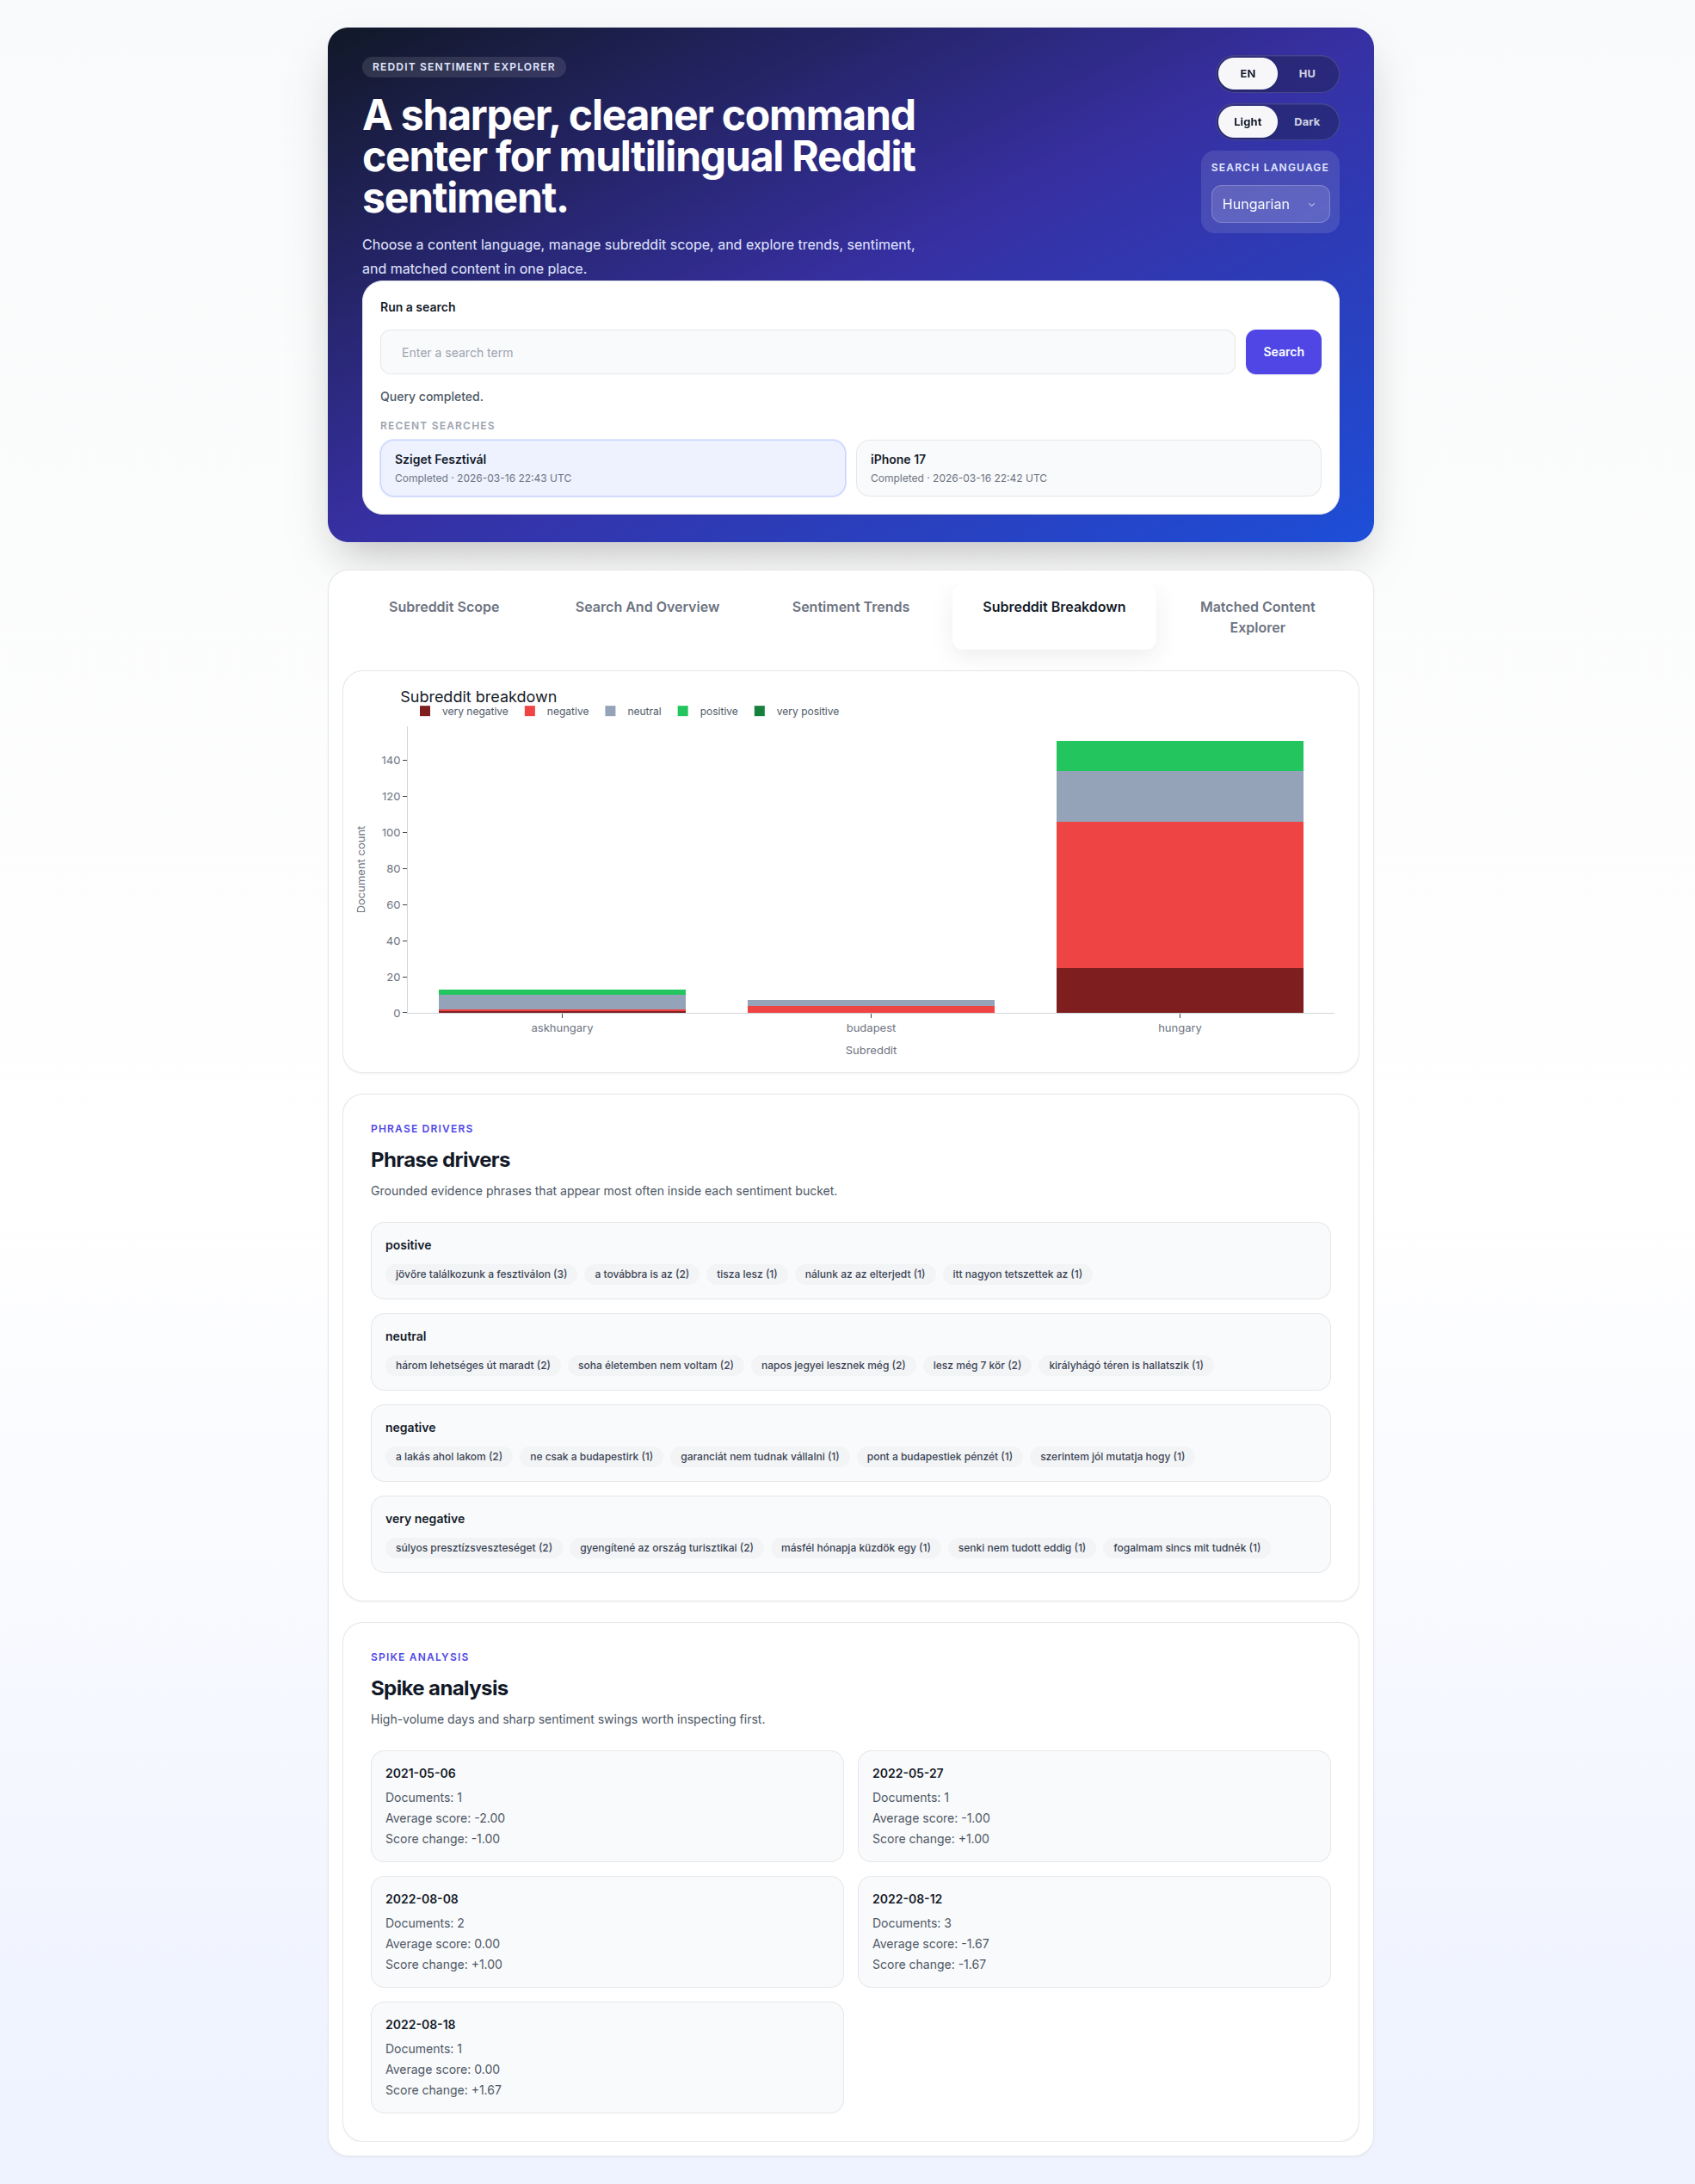
\includegraphics[width=\textwidth]{figures/subreddit-breakdown.png}
    \caption{Subreddit Breakdown tab with per-subreddit chart, phrase drivers, and spike analysis.}
    \label{fig:appendix_breakdown}
\end{figure}

\begin{figure}[H]
    \centering
    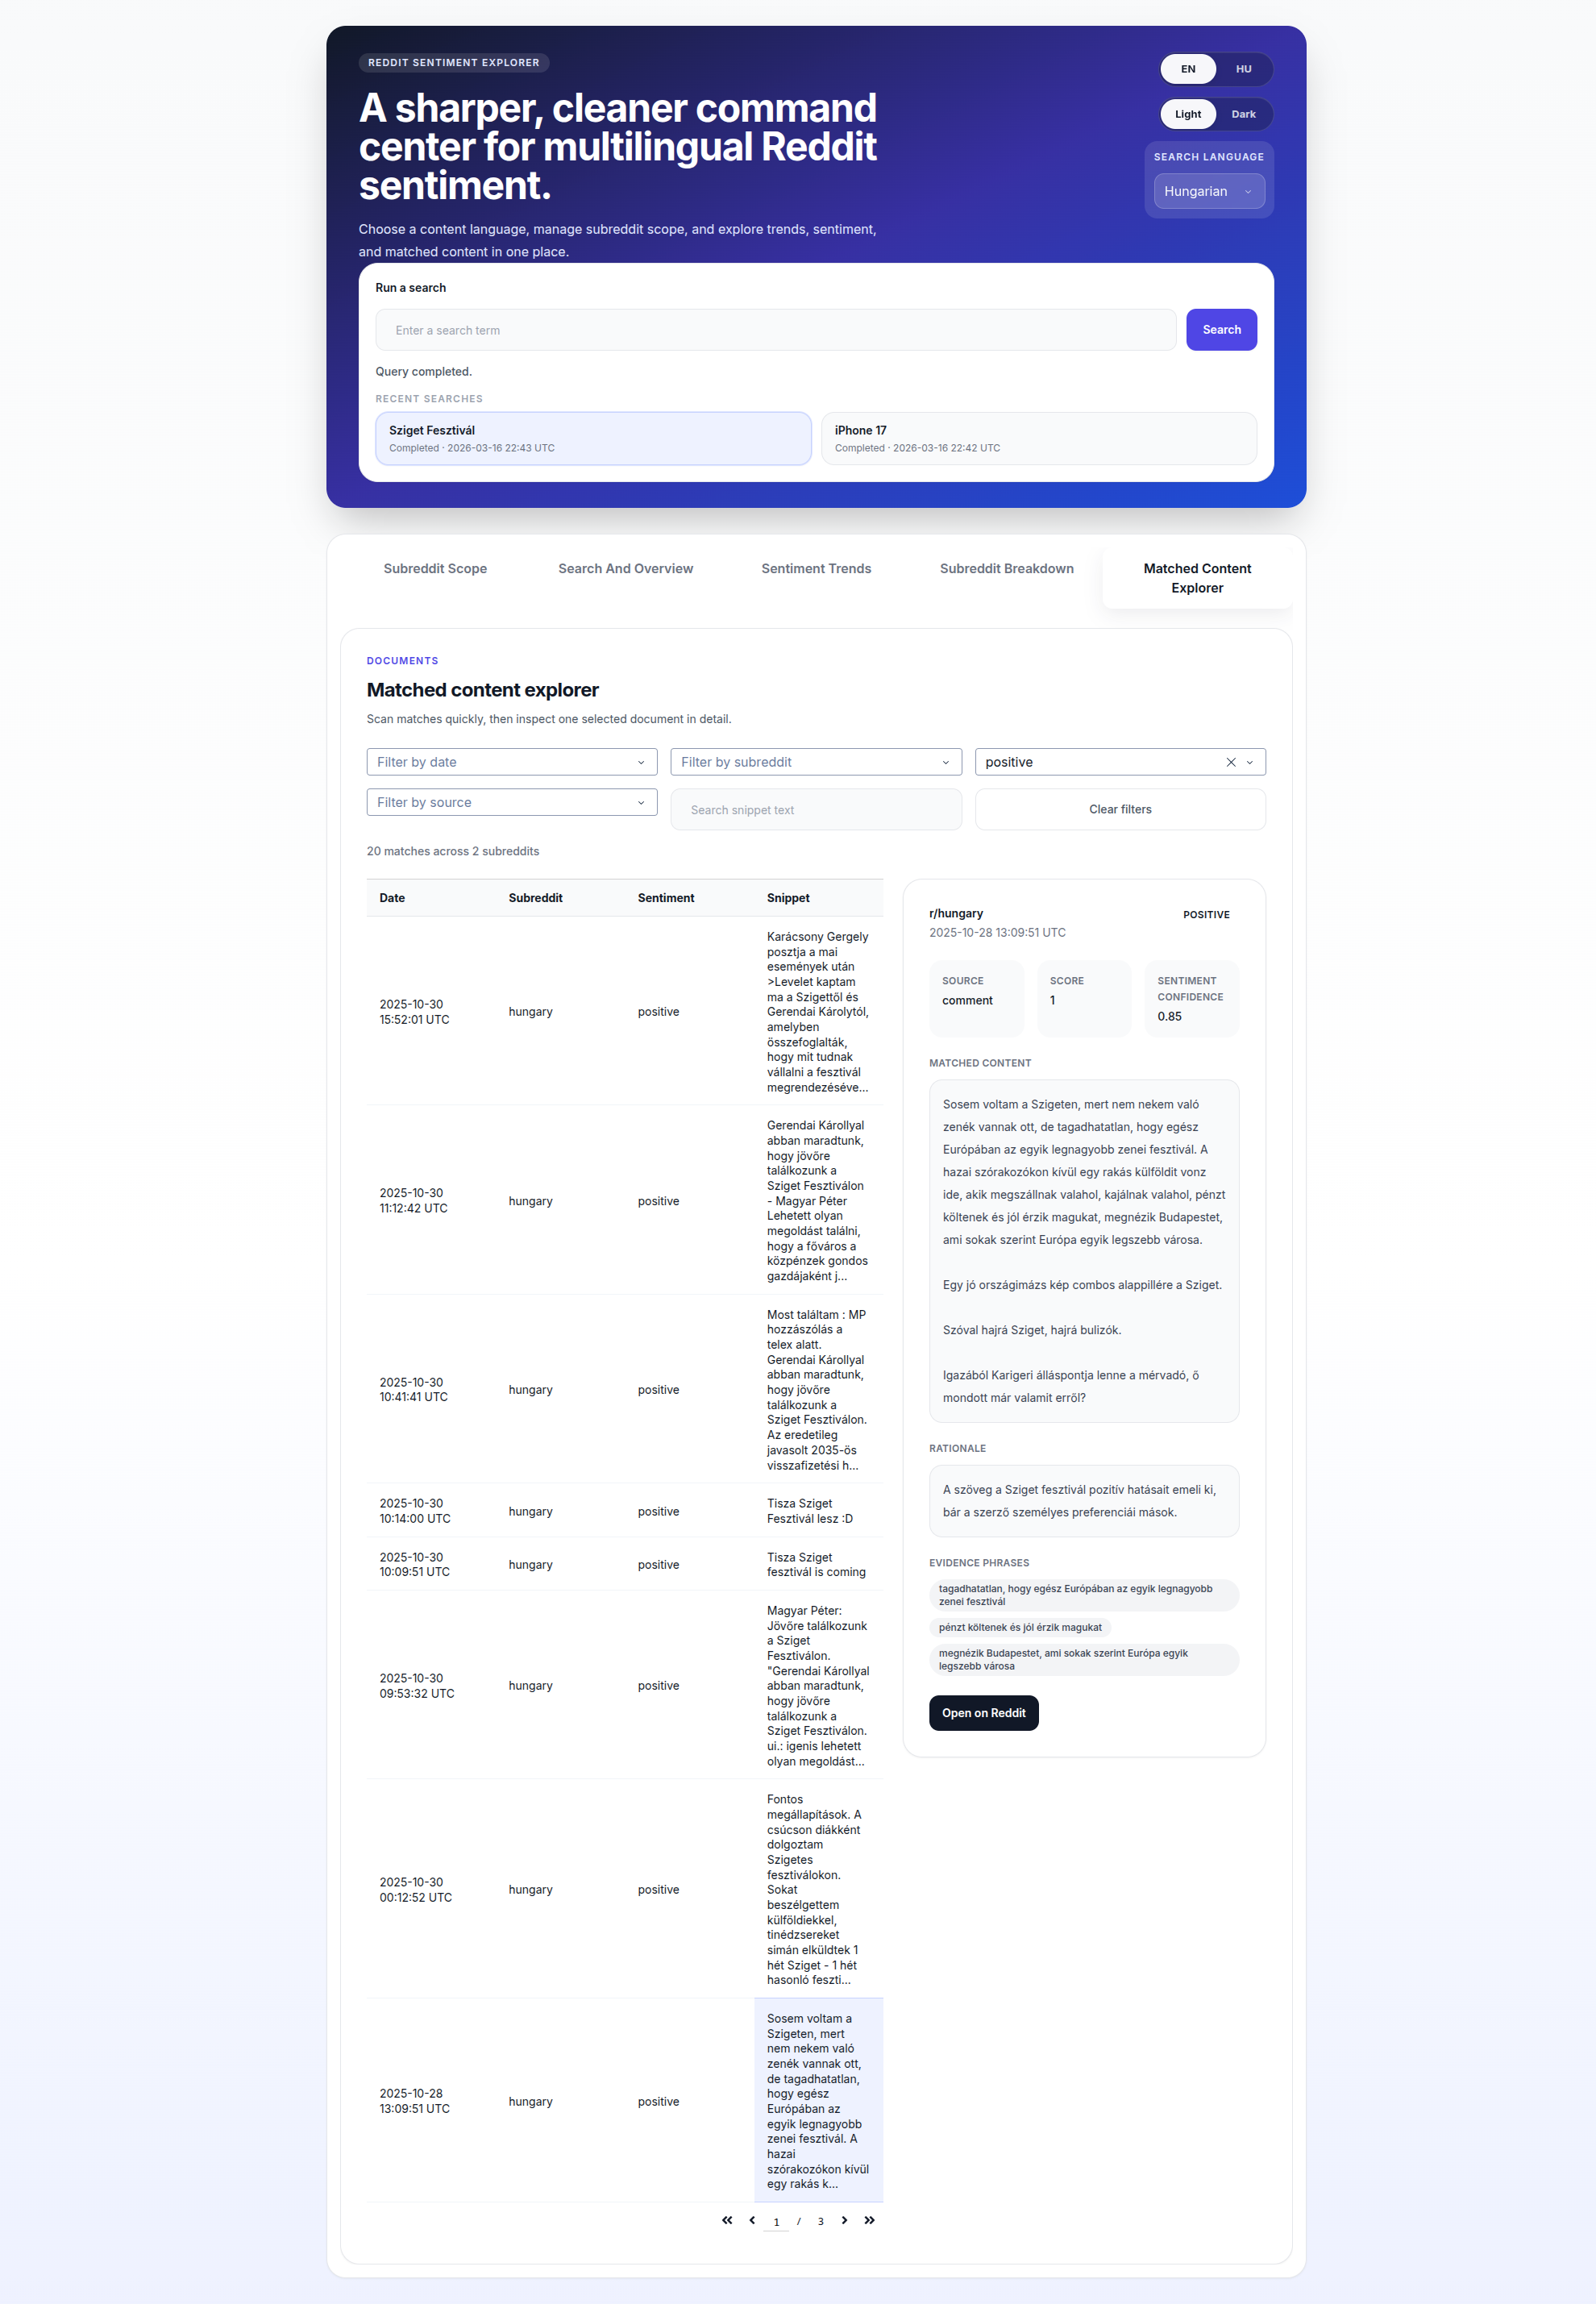
\includegraphics[width=\textwidth]{figures/matched-content.png}
    \caption{Matched Content Explorer with document details, sentiment rationale, and evidence phrases.}
    \label{fig:appendix_matched}
\end{figure}
